\documentclass{article}
\usepackage{tikz}
\usetikzlibrary{arrows,shapes,automata,petri,positioning,calc}
\tikzset{
	place/.style={
		circle,
		thick,
		draw=black,
		fill=gray!50,
		minimum size=6mm,
	},
	state/.style={
		circle,
		thick,
		draw=blue!75,
		fill=blue!20,
		minimum size=6mm,
	},
}

\begin{document}
	
	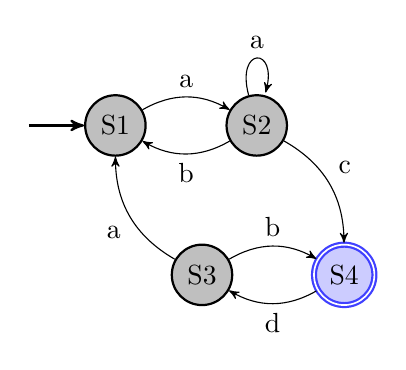
\begin{tikzpicture}[node distance=2cm and 1cm,>=stealth',auto, every place/.style={draw}]
		\node [place] (S1) {S1};
		\coordinate[node distance=1.1cm,left of=S1] (left-S1);
		\coordinate[node distance=1.1cm,right of=S1] (right-S1);
		
		\draw[->, thick] (left-S1) -- (S1);
		
		\node [place] (S2) [right=of S1] {S2};
		\node [place] (S3) [node distance=1.5cm,below =of right-S1] {S3};    
		\node [state,initial text=,accepting by double] (S4) [right=of S3] {S4};
		
		\path[->] (S1) edge [bend left] node {a} (S2);
		\path[->] (S2) edge [bend left] node {b} (S1);
		\path[->] (S2) edge [loop above] node {a} ();
		\path[->] (S3) edge [bend left] node {a} (S1);
		\path[->] (S2) edge [bend left] node {c} (S4);
		\path[->] (S3) edge [bend left] node {b} (S4);
		\path[->] (S4) edge [bend left] node {d} (S3);      
	\end{tikzpicture}
\end{document}
Output
\end{document}
